%%%%%%%%%%%%%%%%%%%%%%%%%%%%%% -*- Mode: Latex -*- %%%%%%%%%%%%%%%%%%%%%%%%%%%%
%% project-relatedwork.tex -- 
%% Author          : Philip Johnson
%% Created On      : Thu Oct  4 08:05:31 2001
%% Last Modified By: Philip M. Johnson
%% Last Modified On: Thu May 26 09:42:41 2005
%% RCS: $Id$
%%%%%%%%%%%%%%%%%%%%%%%%%%%%%%%%%%%%%%%%%%%%%%%%%%%%%%%%%%%%%%%%%%%%%%%%%%%%%%%
%%   Copyright (C) 2001 Philip Johnson
%%%%%%%%%%%%%%%%%%%%%%%%%%%%%%%%%%%%%%%%%%%%%%%%%%%%%%%%%%%%%%%%%%%%%%%%%%%%%%%
%% 
\section{Related Work}

\subsection{Qualitative and quantitative data and its integration}

A primary requirement for Cedar is to support collection, analysis, and
integration of qualitative and quantitative empirical data.  To understand
our approach to this requirement, it is useful to first introduce what we
mean by qualitative and quantitative data and their interrelationship.

{\bf Concepts.} By qualitative data, we mean text, images, and other
materials that have symbolic meaning for some cultural group. Qualitative
data comes in many different forms, from structured interviews, to surveys
and questionnaires, to life history narratives, to full blown cultural
ethnography.  Qualitative data is often textual, but may include graphics,
audio, video, or even clothing, architecture, and other cultural artifacts.

By quantitative data, we mean numbers: interval or ratio measures,
including counts or frequencies of occurrence of objects or events, as well
as the variable properties of those objects or events.  For example, one
might count the number of people on a team, or the number of tasks they
perform per unit time. One might also measure their average tenure in their
current jobs.  In the domain of software engineering, typical quantitative
data might include the number of lines of code (LOC) in a software module,
or the number of modules in a system. Quantitative data always has an
explicit or implicit time dimension: it quantifies something at a given
point or interval in time.  Quantitative data can be derived from
qualitative data. For example, one might count the occurrences of a
particular behavior recorded in a researcher's field notes. 

Of course, numbers do not speak for themselves. Like qualitative data, they
derive meaning from context.  For example, is 5 defects per 1000 lines of
code high or low? Is a \$100,000 error in a financial statement
``material'' or not?  While numbers might seem objective, qualitative data is
often essential to making sense of quantitative data.  The great strength of
qualitative research is its ability to introduce context into the study of
a particular phenomenon.  From the beginning of the research process
(research design, access to research sites, data gathering) to the end
(analysis, writing and publication) qualitative research both necessitates
and enables attention to context.

PI Feldman has carried out a variety of research focused on the question
of how to define systems of meaning from qualitative and quantitative data
\cite{Feldman95,Feldman04}.  Her research illustrates how the analysis of
qualitative data always involves at least two systems of meaning: that of
the subjects being studied (the ``participants'', sometimes called
``natives'' or ``insiders''), and that of the researchers, who have a
theoretical framework.  The participant perspective is referred to as
``emic'', while the researcher perspective is called ``etic''
\cite{Headland90}. Within an organization, there may be several different
``insider'' perspectives, as well.

People, including researchers, often make sense of the world and their
place in it as a form of ``narrative''
\cite{Bruner90,Gee86,Riessman93,Mishler86,Abbott91,White92,Ricoeur81}.
Narrative provides context: it reveals what is significant to people about
various practices, ideas, places, and/or symbols \cite{Young96}.  Narrative
structure can form the basis for an analytical framework that connects the
actions and events with the meaning(s) that these actions have for the
people who take them \cite{Bal85}.  With appropriate representational
support, narrative structure appears promising as a means to integrate
qualitative and quantitative data.  

In summary, we believe that proper interpretation of qualitative and
quantitative data requires context, that the data and context together form
one or more systems of meaning, and that narrative structure forms an
approach to integrated representation of qualitative and quantitative data.
With these concepts in hand, we next review research related to
technological support for collecting, analyzing, and integrating
qualitative and quantitative data.

{\bf Qualitative data collection tools.}  The very nature of qualitative
data limits the kinds of tool support for its collection.  Diaries, field
notes, interviews, and so forth can be readied for analysis with software
for automated transcription or handwriting recognition.  Questionnaires can
be provided in an electronic form, such as over the internet. For example,
Net-MR supports online surveys in 35 languages for multi-country data
collection.

The state of the art in automated coding and analysis systems is advancing
rapidly. For example, the Kansas Event Data System (KEDS) parses newspaper
articles on political events in the Middle East and subjects to extracted
event data to statistical analysis with the goal of predicting political
change in the region \cite{keds}. In research for the National Gallery of
the Spoken Word, researchers are using hidden markov models (HMM) for
speaker-independent keyword recognition. By adding meta-data (codes) to raw
data, these systems prepare qualitative data for subsequent analysis.

{\bf Qualitative analysis tools.} Qualitative analysis tools are generally
of two types: coding support tools and text mining tools.  Coding support
tools, such as ATLAS.ti, MAXqda, N6, NVivo, ETHNO, and Qualrus, allow
researchers to annotate textual or video data with the goal of identifying
the meanings implicit or explicit in the data. These tools help to speed
analysis without disconnecting the data from the context more than is
necessary.  In general, current qualitatitive analysis tools are designed to support a
small team of researchers working with a relatively small set of data
(e.g., a set of interviews or fieldnotes).  They do not support integration 
of quantitative data, support for large-scale distribution, analysis, or 
dissemination, or flexible privacy protection mechanisms.

{\bf Quantitative data collection tools.} Collection of quantitative data
is generally more amenable to automated support than qualitative data.
Through the NSF sponsored Hackystat Project, PI Johnson has been
investigating ``sensor-based'' approaches to automated, unobtrusive
collection of quantitative data regarding software development products and
processes.  Hackystat is based upon his prior research on the Personal
Software Process, which identified both logistical and quality problems
with manual collection and analysis of quantitative software engineering
data \cite{csdl2-01-12,csdl2-02-07}.

Hackystat sensors are small, custom software ``plug-ins'' to developer
tools such as editors, testing tools, configuration management systems,
build tools, and so forth. Once a sensor is installed, it monitors the use
of the tool and automatically sends these raw process or product data to a
web server where further analyses can be performed.  Examples of sensor
data include: activities (compilation, file editing, etc.) within an
editor, invocation of unit tests and their results, size/complexity of the
system (in LOC, methods, classes, operators), configuration management
events (such as commits and lines added/deleted), test case coverage,
software review data (time spent doing review, issues generated, etc.) and
defect management data.  Specialized configurations of Hackystat have been
developed for a variety of contexts, including classroom settings to
support Java development \cite{csdl2-03-12}, at the Jet Propulsion
Laboratory to analyze workflow \cite{csdl2-03-07}, and in case studies of
high performance computing \cite{csdl2-04-22}.  Figure \ref{fig:dailydiary}
illustrates the Daily Diary, one of the perspectives provided by Hackystat
for viewing sensor data. This Daily Diary instance is configured to show
the commands entered by this developer into a shell and the most actively
edited file (if any) during each five minute interval. 

\begin{figure*}[ht]
  \centering
  \includegraphics[width=0.75\textwidth]{truss.commandlineinvocations.eps}
  \caption{Hackystat Daily Diary, illustrating an event stream (shell commands) 
and quantitative data (most actively edited file during a five minute interval)}
  \label{fig:dailydiary}
\end{figure*}

The automated nature of quantitative data collection in Hackystat
allows any single installation to scale to dozens or hundreds of users.
For example, the public Hackystat server maintained at the University of
Hawaii contains accounts for over three hundred users and over 10,000
developer days of data. However, Hackystat does not support qualitative
data collection, and implements a static privacy policy.  

{\bf Quantitative analysis tools.}  Excellent tools exist for the analysis
of quantitative data is through variance-based models, such as regression,
structural equation modeling, event history, and so on.  In the familiar
regression framework, we create a model of the form Y = f(X), which posits
a functional relationship between a set of antecedents (x1, x2, x3, ... xn)
to a set of outcomes (y1, y2, y3, ... ym).  Since all the variables can be
expressed with numbers, we can use covariance-based methods to estimate the
relationships and test their statistical significance.  In software
engineering, for example, the COCOMO cost model predicts outcomes
concerning the cost and time associated with a software project given
antecedents characterizing the system to be built and the resources
available for its construction \cite{Boehm00}.

{\bf Integrating qualitative and quantitative data.} In variance models,
causal mechanisms are usually implicit
\cite{Abbott91,Lawrence97,Griffin93}.  Our quantitative methods allow us to
demonstrate that Y = f(X), but documenting the chain of events that
connects X and Y requires qualitative (narrative) analysis
\cite{Abbott91,Griffin93,Corsaro90,Heise89}. Abbott has argued that
significant new insights can be gained by using narrative models to
investigate the patterns of events or actions that connect important
antecedents and outcomes \cite{Abbott90a, Abbott91,Abbott95}. This insight
forms the basis for our proposed approach to the integration of qualitative
and quantitative data.  PI Johnson has demonstrated this approach in the
analysis of quantitative data in Hackystat called ``Software Project
Telemetry'' \cite{csdl2-04-11}.  Instead of building a predictive model to
connect antecedents to outcomes, telemetry-based analyses focus on
in-process monitoring of data streams and their relative change over time.
For example, if test coverage values begin to trend downward and at the
same time defect reports begin to trend upward, the project managers might
hypothesize that a deterioration in testing quality is making an observable
impact on software quality.  Ongoing research is evaluating Software
Project Telemetry for decision-making in the context of a daily build
process.  Figure \ref{fig:telemetry} shows an example of software project
telemetry which charts the relative growth of serial and parallel lines of
code in a high performance computing application over a 12 month period.


\begin{figure*}[ht]
  \centering
  \includegraphics[width=0.75\textwidth]{parallelsloc.eps}
  \caption{Example Hackystat Telemetry, showing trends in the amount of parallel and serial code 
in a high performance computing application over 12 months}
  \label{fig:telemetry}
\end{figure*}

{\bf Modes of integration.}  Our approach supports three basic modes of
integrating qualitative and quantative data, each of which has significant
body of related work in the social and organizational sciences.

(1) Counting and aggregating. Given a stream of qualitative (or
quantitative) data stored in Cedar, such as events, they can be counted and
aggregated in various ways.  This is a familiar analytical technique, and
we do not see it as a significant research issue.

(2) Identification of causal patterns. Because Cedar will store sequences
(streams) of events, it should support efforts to identify patterns of
events and determine the chain of events that connect antecedents and
consequences. Similarly, optimal string matching
\cite{Abbott83,Abbott90a,Abbott90b,Abbott95,Sabherwal93} has been applied
to a variety of organizational situations. PI Pentland has applied string
matching to actions in a work process, using algorithms developed in
molecular biology for the analysis of genetic sequences to compare and
cluster sequential patterns \cite{Pentland03b}.  Event structure analysis
(ESA)
\cite{Heise89,Corsaro90,Griffin93,Griffin94,Stevenson03,Stevenson98,Stevenson00}
provides another methodology for interpreting events captured in
ethnographic fieldnotes in terms of coherent patterns.
 
(3) Contextualization and interpretation.  As mentioned above, traditional
qualitative analysis requires putting data in context.  The representation
we propose to develop for Cedar (discussed below) will allow users to
analyze qualitative and quantitative data using network techniques.
Network representations provide a powerful means of contextualizing and
interpreting qualitative data, as in semantic networks
\cite{Sowa84,Carley97}, ``cause maps'' \cite{Nelson91,Bougon77} and
``networks of action'' \cite{Czarniawska97,Pentland99a,Abell87}.  PI
Pentland has investigated the use of network models to represent
interaction processes, and has developed a conceptual framework for the use
of narrative data in the analysis of organizational processes
\cite{Pentland03a,Pentland99a}.

{\bf Research Issues.} Prior research indicates the promise of event-based
analysis of qualitative and quantitative data, both separately and
together.  However, the research and technological innovations to date has
been fragmented, both by discipline and by application area.  Qualitative
analysis techniques cannot scale to analysis of dozens or hundreds of
subjects supported by Hackystat.  On the other hand, the interpretation of
event-based data collected by Hackystat could be improved by the narrative
and network modeling techniques available from social science research.
Finally, all of the research and technology suffers from an inability to
interoperate with each other.


\subsection{Infrastructure and experimental data repositories}
\label{sec:repositories}

An important component of empirical study is the generation of data,
artifacts, and the use of experimental testbeds of various
kinds. Infrastructure, such as online data repositories, makes this
information available to others in the community to enable experimental
replication, meta-analysis, and other applications.  In this section, we
present some examples of prior work on infrastructure and experimental data
repositories for empirical research, followed a summary of the common themes. 

{\bf NASA SEL database.} Since its inception in 1976, PI Basili has been
affiliated with the NASA Software Engineering Laboratory (SEL).  The
original mission of SEL was to study software development for Ground
Support Software at NASA/GSFC with the goal of improving the quality of the
software developed \cite{Basili95}. The lab has collected a variety of case
study data including: resource usage; changes and defects; process,
project, and product characteristics; and process conformance on several
hundred projects.  The artifacts developed are production ground support
systems for NASA missions.  Models of cost, schedule, and quality were
built using this data.  For years, this data was given away freely and made
available through two repositories, one at NASA and one at the Rome Air
Development Center.

Issues with the SEL experimental data repository experience include: misuse
and misinterpretation of the data due to a lack of context information,
leading to publications with questionable results; secondary data analyses
were not known or shown to SEL; overhead of organizing, publishing, and
supporting the repository; lack of support for feedback and meta-analysis.
repository.  Late in the life cycle of the project, it was recommended that
anyone who wanted to use the data must first spend some time at the SEL in
order to acquire an understanding of the nature of the data and its
appropriate use.

{\bf CeBASE.} More recently, PI Basili (along with Barry Boehm of USC)
developed the Center for Empirically-based Software Engineering
(CeBASE). CeBASE is an NSF sponsored project with the role of acting as a
repository of "experience" on the effects of applying a variety of
techniques, methods and life-cycle models to software development. Initial
focus areas are defect detection methods \cite{Boehm01}, COTS development
\cite{Basili01}, and Agile methods. Data available in CeBase is currently 
qualitative in nature and is manually organized by the website maintainers.
While CeBase contributors become publically affiliated with the project, as
with the SEL repository, the data is made publically available from the
website and there is no monitoring or control over dissemination.

Although CeBase is a much younger repository than SEL, many of the same
issues regarding appropriate use of the data are expected to apply: how 
to ensure that secondary analyses of data is done appropriately, and how to 
support the ongoing overhead of repository maintenance and support. 

{\bf Hackystat.} As noted in the previous section, PI Johnson has been
leading the Hackystat Project, which supports automated collection and
analysis of quantitative software engineering data and which produces an
information repository suited to empirical experimentation. The Hackystat
data repository contrasts in an interesting way with both the SEL or CeBase
repositories. While SEL and CeBase repositories are populated by data from
completed projects or case studies, the Hackystat data repository collects
data incrementally, in real-time, as a project progresses.  While access to
the information in the SEL and CeBase repositories is unlimited and
uncontrolled, access to Hackystat data is strictly controlled: only the
data owners or members of the project can access the data and use it for
empirical analyses of their projects. For this reason, a central issue for
the Hackystat data repository is effectively the opposite confronted by SEL
and CeBase: how to make the Hackystat data public, and what form should
that public data take?

{\bf Other experimental data repositories.}  Hackystat, SEL, and CeBase
illustrate some of the experimental data repositories with which the PIs
have had direct experience, but other repositories exist.  For example,
TheDataWeb is an online information repository for demographic, economic,
environmental, health, and other datasets.  Developed through a
collaboration between the U.S. Census Bureau and the Centers for Disease
Control, TheDataWeb provides unified access to data housed in different
systems in 16 different federal agencies. Example datasets include American
Housing Survey, the Behavioral Risk Factor Surveillance System, the
Consumer Expenditure Survey, the Current Population Survey, and the
National Center for Health Statistics Mortality Survey.  From an
implementation perspective, TheDataWeb consists of two parts: a ``DataWeb
Servlet System'', which providers of data can use to make their datasets
accessable to users of the TheDataWeb, and the ``DataFerrett'', a
client-side application that enables users to browse and query these
datasets and extract data from them.

{\bf Research Issues.}  A central theme from the research to date on
experimental data repositories is the importance of flexible control over
access and dissemination of experimental data.  In the case of SEL, too
much access has led to inappropriate use of the experimental data and
publication of questionable results.  In the case of Hackystat, the
fine-gained nature of the data and presence of personally identifying
information has resulted in a policy of too little access, such that this
rich source of experimental data is not available for secondary analysis,
meta-analysis, replication, and so forth.  Finally, lack of communication
mechanisms between these repositories limits the possible insights to be 
gained by data aggregation and meta-analysis.

\subsection{Privacy policies}
\label{sec:privacy}

As the prior section demonstrates, an important unsolved question in
experimental data repositories is how to control the access and
dissemination of the stored data.  Such privacy policies must take into
account a variety of issues. 

The first, and most obvious issue, is to protect the privacy of the
participants providing data to the repository.  Singer provides an
excellent overview of the ethical issues involved with data collection and
storage of human subject data from empirical studies \cite{Singer02}.  She
analyzes the literature on research ethics and identifies four general
principles for ethical empirical experimentation: informed consent,
scientific value, beneficence, and confidentiality, and illustrates their
application or misapplication in a variety of experimental contexts.

Singer makes the important point that compromising these guidelines not
only risks the exploitation of individuals associated with the study, it
also risks harming the study, the subjects themselves, or the organization
under study.  For example, missing or insufficient application of informed
consent or confidentiality could lead to subjects not cooperating or
providing incorrect data.  In the case of their managers, it could lead to
loss of access to study sites or loss of funding. Both of these harm the
study.  Inappropriate access to empirical data could reveal data that could
be used to damage an individual's professional reputation, harming their
career. Finally, inappropriate interpretation of data could lead to
negative consequences for the organization in which the study took place.
Austen provides an additional perspective on this kind of institutional
harm called ``measurement dysfunction'' \cite{Austen96}.  Such ``secondary''
use of data and its privacy implications have been investigated in a health
care setting \cite{Lowrance03}.

Singer applies the principles of informed consent, scientific value,
beneficence, and confidentiality somewhat narrowly to the subjects and
organizations who provide the data to the repository.  Our prior
involvement with public data repositories reveals the need to expand these
principles in our proposed research.  For example, the SEL experience
demonstrates the real risk that public repositories of empirical data can
lead to misinterpretation of the extracted data due to inadequate
contextual information (i.e. meta-data). Our Hackystat experience
demonstrates that ``boilerplate'' application of standard informed consent
practices in an educational setting leads to a repository whose data cannot
be effectively ``freed'' for purposes such as third-party meta-analysis.
The presence of an online, publically available data repository creates the
need for privacy policies that enable control not only over the type and
level of contributions to the database by subjects, but also on the type
and level of data extracted from the database by users.  Indeed, for a
long-lived data repository, such control might evolve over time: data
contributed regarding an organizational project might have quite restricted
access at the time it is initially contributed due to risks of leaking
proprietary data.  Five or ten years later, a more relaxed level of control
over access might be possible, rendering new types of analysis possible.  

Some prior work has been done on the technology of privacy specification
and implementation. For example, the Platform for Privacy Preferences
project has developed a way for users to specify and change their privacy
preferences with respect to their interactions over the Internet
\cite{Cranor03}, though other research has indicated that what people
specify as their preferences may not reflect their actual behavior
\cite{Spiekermann01}. Research is also available on sanitizing or
anonymizing private data for the purpose of data mining \cite{Rizvi02,
Iyengar02}. These approaches typically involve perturbation of data values,
generalization/abstraction, or suppression.  

{\bf Research issues.}  To build an effective
cyberinfrastructure for qualititative and quantitative data collection and
analysis, we must be aligned with the four principles of research ethics,
expand them to address control over collection and dissemination and its
evolution over time, and leverage the technology that is currently
available.

\subsection{Results from prior NSF research}

\small
\begin{tabular}{lp{4.5in}}

Award number: & CCF02-34568 \\
Program: & Highly Dependable Computing and Communication Systems Research\\
Amount: & \$638,000 \\
Period of support: & September 2002 to September 2006 \\
Title of Project: & Supporting development of highly dependable software through
continuous, automated, in-process, and individualized software measurement validation \\
Principal Investigator: & Philip M. Johnson \\
Selected Publications: & \cite{csdl2-04-22,csdl2-04-13,csdl2-04-11,csdl2-03-12,csdl2-02-07,csdl2-03-07,csdl2-04-02,csdl2-04-04,csdl2-04-06}
\end{tabular} \\ %[3mm]
\normalsize

\medskip

The general objective of this research project is to design, implement, and
validate software measures within a development infrastructure that
supports the development of highly dependable software systems.
Contributions of this research project include: (a) development of a
specialized configuration of Hackystat to automatically acquire build and
workflow data from the configuration management system for the Mission Data
System (MDS) project at Jet Propulsion Laboratory; (b) development of
analyses over MDS build and workflow data to support identification of
potential bottlenecks and process validation; (c) identification of
previous unknown variation within the MDS development process; (d)
development of a generalized approach to in-process, continuous measurement
validation called ``Software Project Telemetry'', (e) substantial
enhancements to the open source Hackystat framework, improving its
generality and usability; (f) development of undergraduate and graduate
software engineering curriculum involving the use of Hackystat for
automated software engineering metrics collection and analysis; (g) support
for 3 Ph.D., 6 M.S., and 3 B.S. degree students. 

\medskip
\noindent
\small
\begin{tabular}{lp{4.5in}}

Award number: & CCR-0086078 \\
Program: & Information Technology Research\\
Amount: & \$2,400,000 \\
Period of support: & September 2000 to September 2003 \\
Title of Project: & ITR: Collaborative Research Proposal for a National Center for Empirical Software Engineering Research\\
Principal Investigator: & Victor Basili, Barry Boehm \\
Selected Publications: & \cite{Basili01b,Basili02b,Boehm02,Jiwnani02,Morisio02,Rus02,Shull02,Shull02b}
\end{tabular} \\[3mm]
\normalsize

The CeBase research activities have allowed the current research team to
build significant expertise in the areas of software engineering decision
support, defect analysis, and empirical study that are vital for the
proposed work. Contributions of this research include: (a) interaction with
an official "affiliates list" of over 21 university, industry, and other
research organizations; (b) Three tutorials in empirical research methods
and empirical results; (c) 11 end-user forums for CeBase end-users; (d)
Development of a publicly-available repository, www.cebase.org, containing
research tools, reusable artifacts and documents, supporting data, and
results. (e) Development and public release of tools (such as eWorkshop)
for use by the empirical research community; (f) 9 books and book chapters,
46 refereed journal publications; 57 refereed conference and workshop
publications; (g) support for 10 Ph.D., 6 M.S., and several B.S. degree students. 


%% \medskip
%% \noindent
%% \small
%% \begin{tabular}{lp{4.5in}}
%% 
%% Award number: & DMI-0075396 \\
%% Program: & Scalable Enterprise Systems \\
%% Amount: & \$146,086 \\
%% Period of support: & September 2000 to December 2001 \\
%% Title of Project: & More is Different - A Grammatical Approach to Scalable Enterprise Systems\\
%% Principal Investigator: & M. J. Chung, P. Kwon, B. Pentland \\
%% Selected Publications: & \cite{Chung02,Chung03,Kwon02,Zeng03}
%% 
%% \end{tabular} \\[3mm]
%% \normalsize
%% 
%% This was an exploratory grant to develop a process management
%% framework for distributed design and manufacturing processes. Contributions
%% of this research include: (a) a XML-based framework for the representation
%% of design and manufacturing process fragments; (b) software for searching
%% and assembling process fragments to create process plans; (c) a run-time
%% environment for supporting the execution of process plans; (d) support for
%% 2 graduate students; and (e) various publications and presentations.







